This chapter presents important research in the realm of OAuth security and intrusion detection using similar techniques as proposed in this work. As one goal of this thesis is to build a strong foundation of the OAuth threat landscape, Section \ref{sec:oauth_security_research} starts by showcasing important publications in the realm of theoretical security of the OAuth 2.0 standard. It then proceeds to present a recent security study on practical implementations of OAuth, which was already mentioned briefly in the introduction

Section \ref{sec:anomaly_based_intrusion_detection} continues with examples of related work, which utilize similar techniques to the ones applied in this work, but in different contexts or based on different dataset approaches.

\section{OAuth Security Research}
\label{sec:oauth_security_research}
In the area of OAuth security, a lot of research focuses on analyzing implementations of the OAuth standard in practice. Surveys scanning public OAuth providers for vulnerabilities exist \cite{philippaerts2022oauch}, as well as analysis of OAuth flows using finite state machines \cite{munonye2022machine}. However, there are publications by one research group, that focus on the OAuth standard itself, which is presented in  Section \ref{subsec:fks_model}, because it had an important impact on the OAuth 2.0 standard itself.

\subsection{Theoretical Security Analysis of OAuth}
\label{subsec:fks_model}
Security research on the OAuth standard has been conducted since its beginnings. Impactful research that unveiled security issues in the definition of OAuth 2.0 is the work by Fett et al. \cite{fett2016comprehensive}, who constructed a theoretical \emph{Dolev Yao}-style model called the \emph{FKS} model and extended that model with OAuth2 capabilities. On the one hand, the FKS model mimics web standards, like HTTP/1.1 and HTML5. On the other hand, it simulates entities like browsers, including the concept of windows, documents, iframes, complex navigation rules, DNS servers, web servers, and web and network attackers. The FKS model puts entities as processes into practice, while the communication through standards is modeled via events between the processes. For OAuth 2.0, the researchers' goal is to reveal security flaws in the most secure implementation of the standard regarding all publicly known security considerations while modeling the four grant types: \emph{implicit grant}, \emph{authorization code grant}, \emph{resource owner password credentials grant}, and \emph{client credentials grant}. The central methodology of Fett et al. is to prove the security of the OAuth standard using their formal language, in which the standard is modeled, to find the flaws breaking the security proof. Following this methodology, the researchers uncovered four new threats in the  OAuth standard, with the impact that the OAuth working group of IETF added these threats and their countermeasures to the official document for security best practices for OAuth \cite{lodderstedt2020oauth}.

\subsection{Analysis of OAuth implementations}
Through research like the one mentioned discussed in Section \ref{subsec:fks_model} by Fett et al. and the continuous work by the OAuth working group of the IETF, the OAuth standard gets enriched with several suggestions for improving the security of OAuth implementations. However, because OAuth is such a complex protocol, implementation flaws still arise, even concerning already-known threats. A recent study by Philippaerts et al. implemented an audit tool called \emph{OAuch} to test the coverage of countermeasures against known threats for OAuth. It revealed that 97 of 100 popular authorization providers (OAuth and Open ID Connect) leave at least one common threat completely unmitigated. The researchers also found that, on average, authorization providers, in particular, did not implement 34\% of the security specifications suggested by the OAuth working group \cite{philippaerts2022oauch}. This work again shows the importance of awareness of the threat landscape when implementing and operating an authorization server or an OAuth client.

\section{Anomaly-based Intrusion Detection}
\label{sec:anomaly_based_intrusion_detection}
In the realm of intrusion detection, anomaly-based intrusion detection is a popular research topic, as this type of detection bears one important advantage. Anomaly-based intrusion detection possibly detects unknown attacks in network traffic. Over the last two decades, research in this area has been conducted on benchmark datasets like the \emph{KDD’99} dataset \cite{kdd1999} and updated versions of it. Even though this work uses a self-simulated dataset, because of the lack of existing OAuth intrusion network data, techniques applied in such research can be transferred to the scenario of this work. Relevant research for these techniques is showcased in the following sections.

\subsection{Word Embeddings for Feature Extraction}
One issue to overcome, when working with data logs is to extract relevant features and convert them into a form, that is digestible for machine learning algorithms. Especially textual data, which may hold semantic meaning poses a challenge in that regard. The research by Corizzo et al. \cite{corizzo2020feature} focuses exactly on tackling this issue, by proposing methods, where raw system calls get encoded by different NLP algorithms. The researchers tested their methods on three different datasets and concluded that an approach combining Word2Vec and TF-IDF performs the best. As visualized in Figure \ref{fig:w2v_feat_extr} even just applying Word2Vec performed in the same area of results as the combination with TF-IDF. Even though the work by Corrizzo et al. concludes that the results are not vast enough, it shows that there is potential in this technique to carry out intrusion detection tasks.

\begin{figure}[H]
	\sffamily\footnotesize
	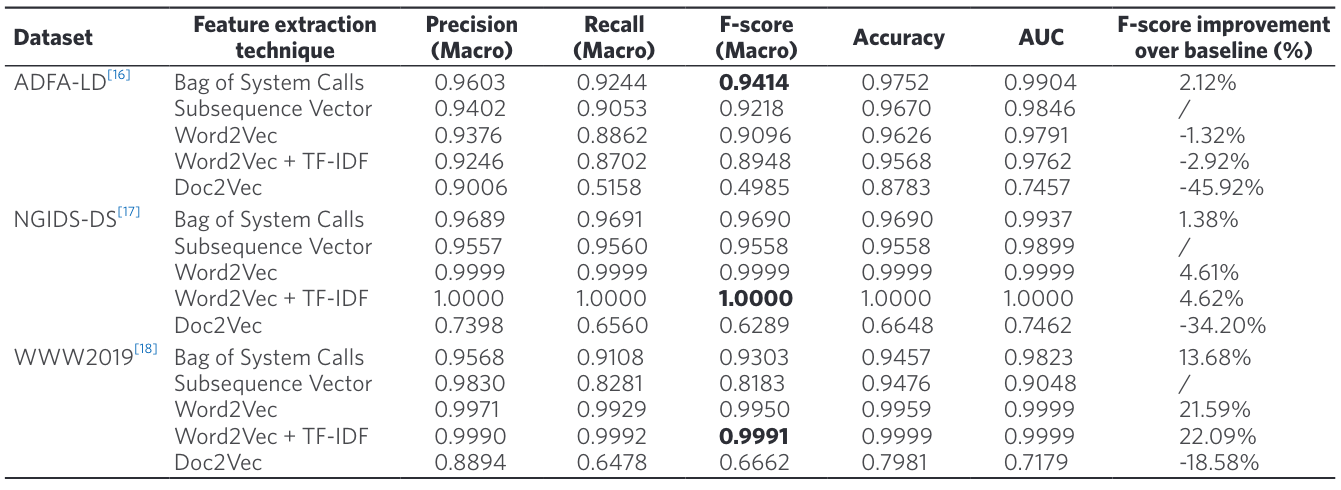
\includegraphics[width=1\textwidth]{pic/w2v_feat_extr.png}
	\unitlength=0.75mm
	\special{em:linewidth 0.4pt}
	\linethickness{0.4pt}
	\caption{Results of applying different NLP techniques for feature extraction on three different datasets of Host-based intrusion data \cite{corizzo2020feature}}
	\label{fig:w2v_feat_extr}
\end{figure}


\subsection{K-Means and Intrusion Detection}
\label{subsec:k_means_intrusion_detection}
Clustering algorithms, like k-means, have had their place in the anomaly-based intrusion detection research landscape for several years. Earlier research focuses on solely applying these algorithms to filter out anomalous traffic by calculating cluster centroids using k-means and measuring the distance from every datapoint to every centroid to determine outliers for anomaly detection \cite{munz2007traffic}. The research by Nalavade et al. \cite{nalavade2014} is an example of applying the k-means algorithm for network intrusion detection again using the famous \emph{KDD`99} dataset \cite{kdd1999}. The researchers preprocess the data by determining features, that hold more relevance than others and increasing their weights for the clustering, by altering their distance metric during clustering. The results depicted in Figure \ref{fig:k_means_navalde} show that Navalde et al. had some success detecting certain types of attacks like Denial of Service. 

\begin{figure}[H]
	\sffamily\footnotesize
	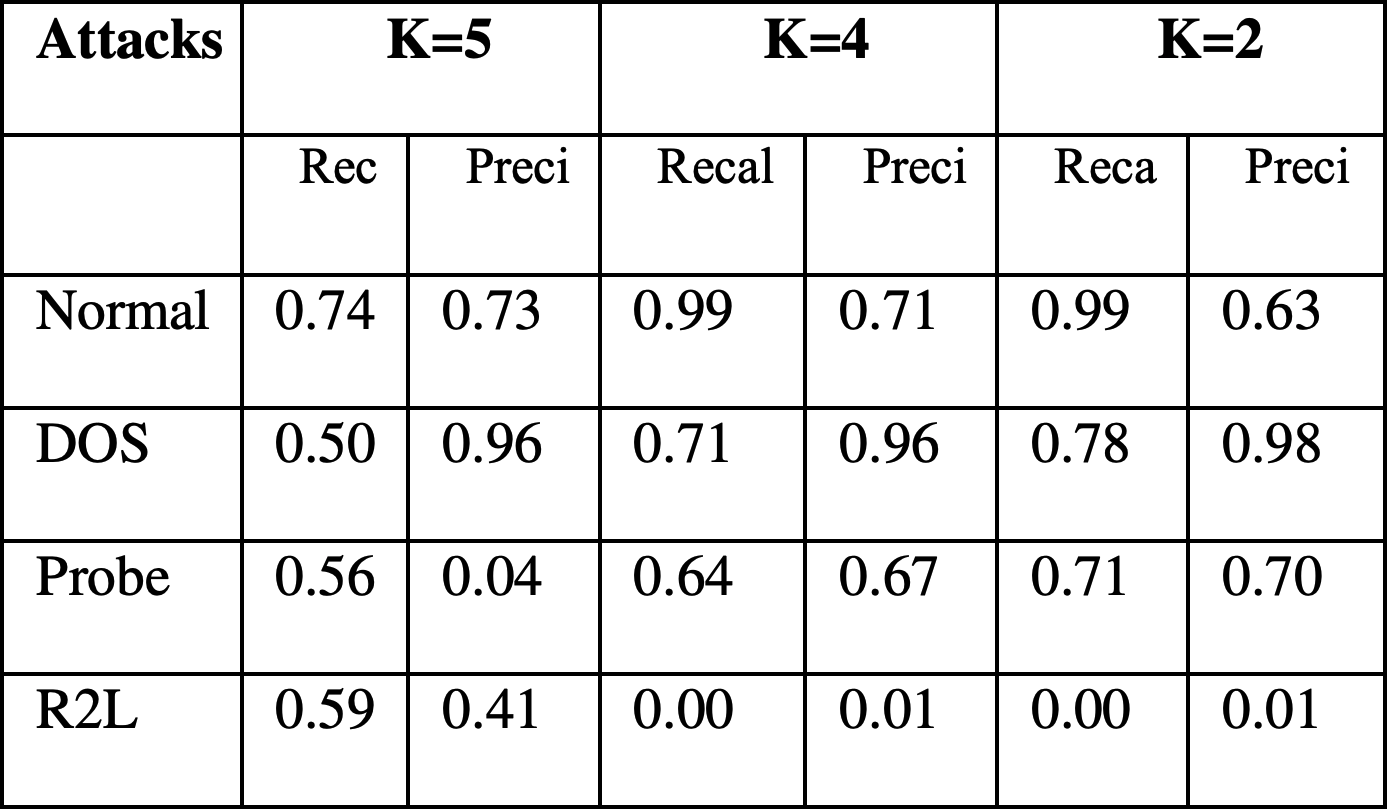
\includegraphics[width=0.5\textwidth]{pic/navalde_k_means.png}
	\unitlength=0.75mm
	\special{em:linewidth 0.4pt}
	\linethickness{0.4pt}
	\caption{Results by Navalde et al. applying k-means for different cluster sizes $K$ to the KDD`99 dataset after pre-processing the data for intrusion detection \cite{nalavade2014}}
	\label{fig:k_means_navalde}
\end{figure}


\subsection{Self-organizing Maps and Intrusion Detection}
Besides k-means other clustering approaches are frequently researched for intrusion detection. One of these other clustering algorithms is the Self-Organizing Maps algorithm. A survey by Qu et al. \cite{qu2021survey} provides a taxonomy of different SOM approaches for network intrusion (see Figure \ref{fig:som_taxonomy}). The researchers present generally three main categories, where static SOMs are not able to adapt dynamically to new input data, whereas dynamic SOMs have this capability. The hybrid SOMs are a combination of SOMs with any other technique. One example of such a hybrid SOM is the combination of SOM and k-means, which improves the overall performance in intrusion detection on the KDD`99 dataset (see Figure \ref{fig:som_kmeans}) based on the results of different studies gathered by the survey. Figure \ref{fig:som_kmeans} also shows that the results for k-means without SOM are significantly better than the results presented in section \ref{subsec:k_means_intrusion_detection}. This further emphasizes that the preprocessing of the data is a very important step for intrusion detection.

\begin{figure}[H]
	\sffamily\footnotesize
	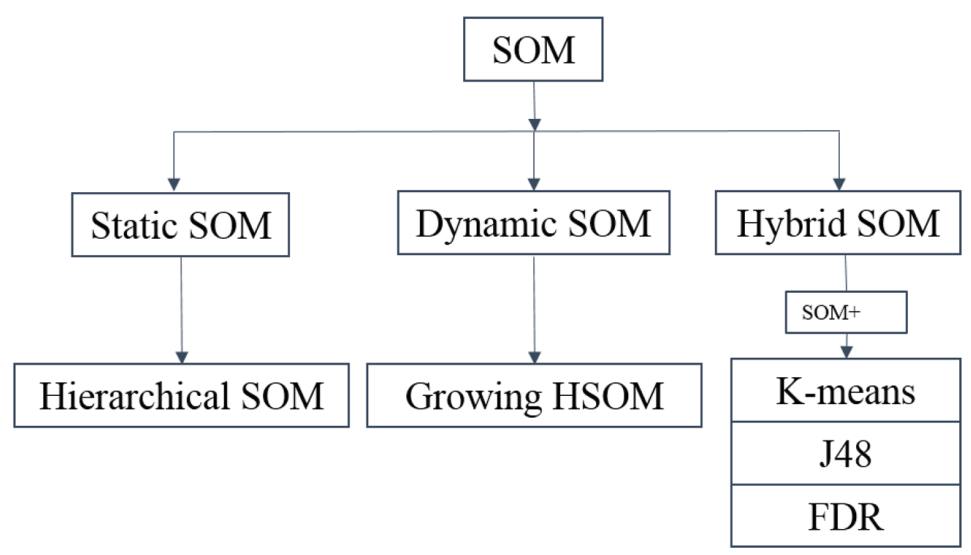
\includegraphics[width=0.5\textwidth]{pic/som_taxonomy.png}
	\unitlength=0.5mm
	\special{em:linewidth 0.4pt}
	\linethickness{0.4pt}
	\caption{Taxonomy of different approaches for implementing Self-Organizing Maps \cite{qu2021survey}}
	\label{fig:som_taxonomy}
\end{figure}

\begin{figure}[H]
	\sffamily\footnotesize
	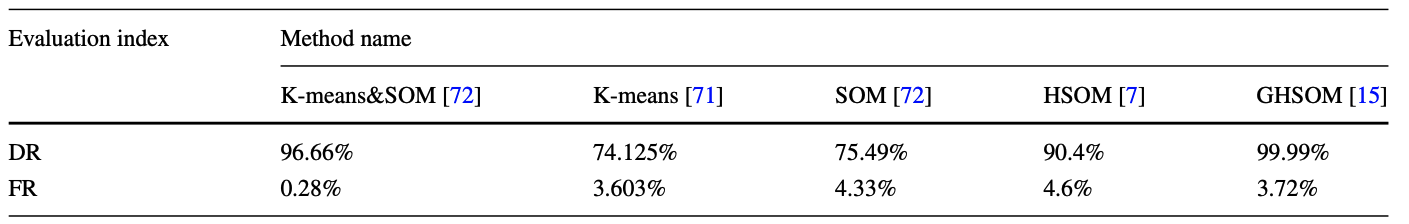
\includegraphics[width=0.9\textwidth]{pic/som_kmeans.png}
	\unitlength=0.5mm
	\special{em:linewidth 0.4pt}
	\linethickness{0.4pt}
	\caption{Results of different research, applying SOM methods for intrusion detection on the KDD`99 dataset (\emph{DR=detection rate, FR=false positive rate}) \cite{qu2021survey}}
	\label{fig:som_kmeans}
\end{figure}